\documentclass[12pt]{article}


\usepackage{amssymb}
\usepackage{amsmath}
\usepackage{fullpage}
\usepackage{epsfig}
\usepackage{epstopdf, xcolor, hyperref}
\everymath{\displaystyle}
\usepackage{enumerate}

\newif\ifans

\anstrue

\begin{document}

\begin{center}
\underline{\LARGE{Double Integrals Over General Regions}}
\end{center}

\noindent SUGGESTED REFERENCE MATERIAL:

\bigskip

\noindent As you work through the problems listed below, you should reference Chapter 14.2 of the recommended textbook (or the equivalent chapter in your alternative textbook/online resource) and your lecture notes.

\bigskip

\noindent EXPECTED SKILLS:

\begin{itemize}

\item Be able to compute double integral calculations over rectangular regions using partial integration. 

\item Know how to inspect an integral to decide if the order of integration is easier one way ($y$ first, $x$ second) or the other ($x$ first, $y$ second). 

\item Kow how to use a double integral to calculate the volume under a surface or find the area or a region in the $xy$-plane.

\item Know how to reverse the order of integration to simplify the evaluation of a double integral.

\end{itemize}

\noindent PRACTICE PROBLEMS:

\medskip

\begin{enumerate}

\item Consider the region $R$ shown below which is enclosed by $y=x^3$, $y=0$ and $x=1$.

\begin{center}
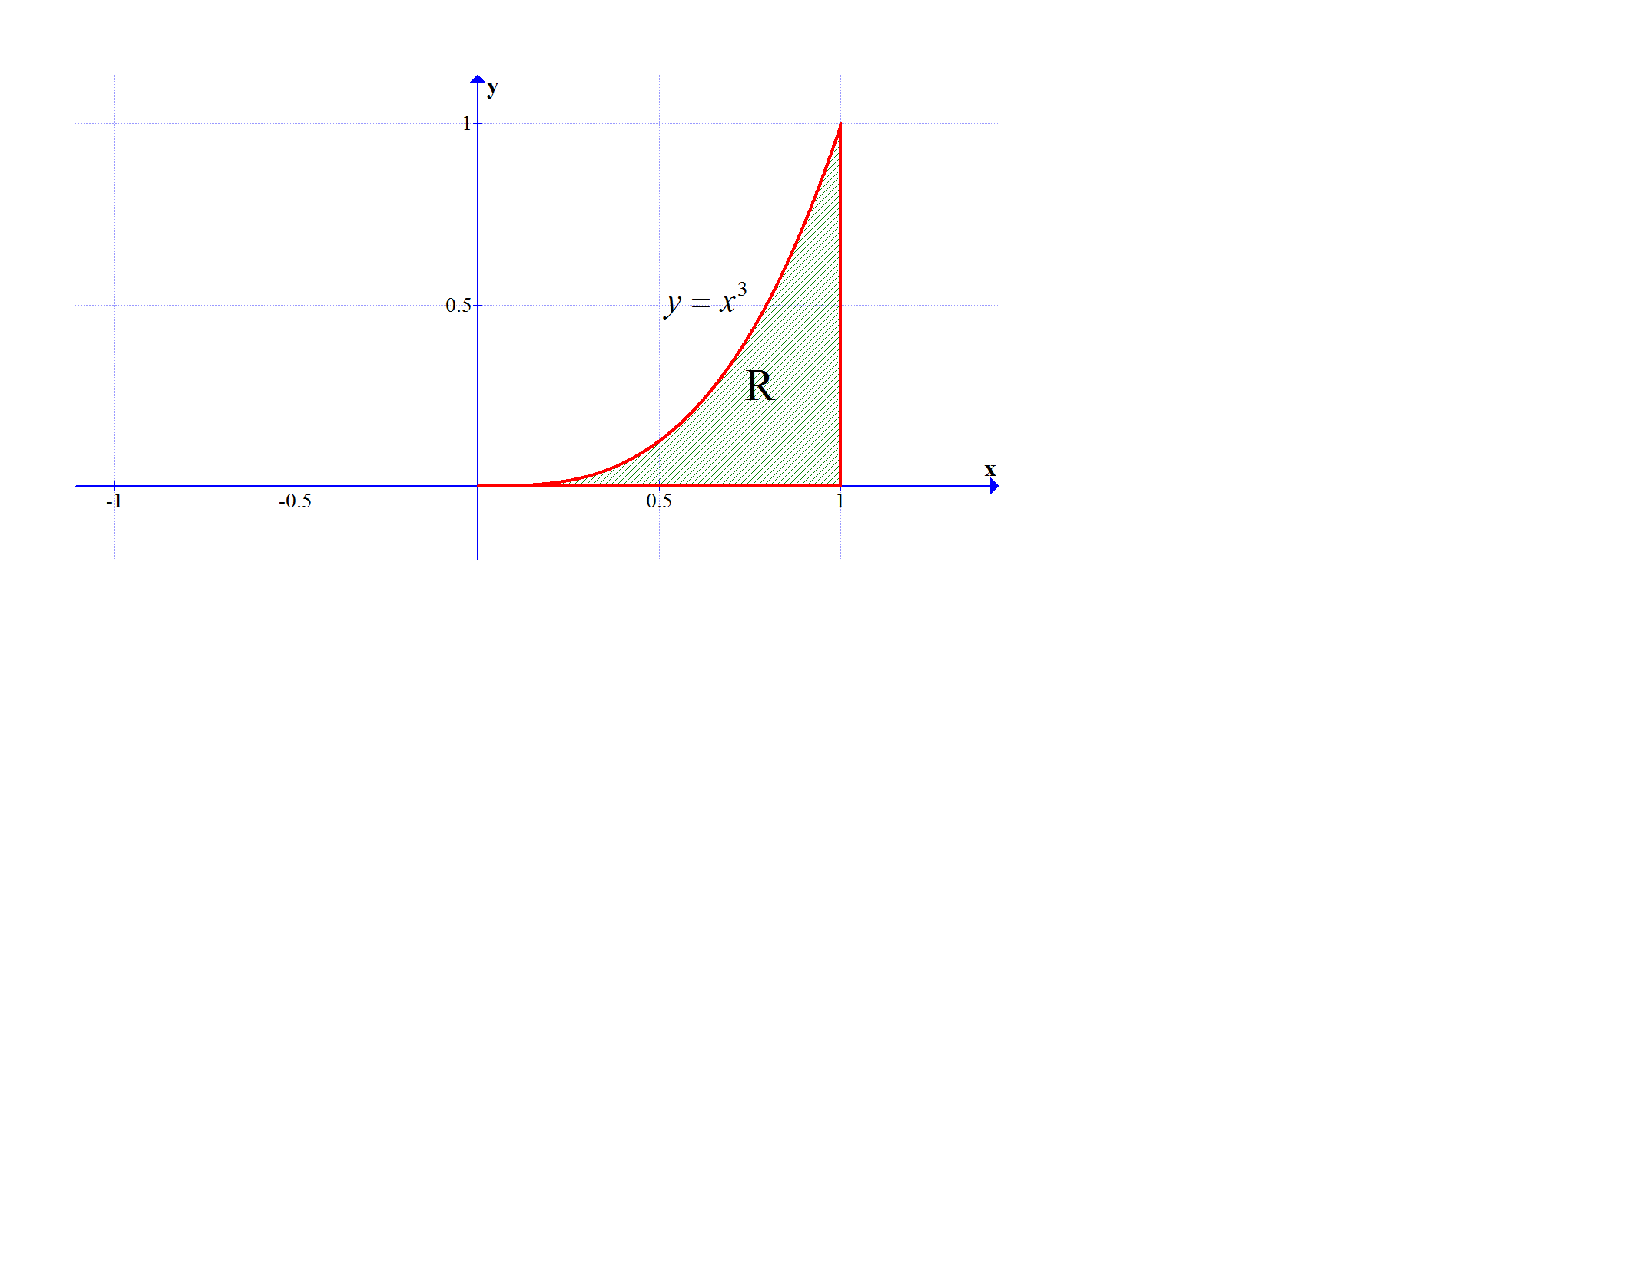
\includegraphics[scale=0.6]{int1.pdf}
\end{center}

Fill in the missing limits of integration.

\begin{enumerate}

\item $\iint \limits_{R} f(x,y) \,dA= \int_{\fbox{}}^{\fbox{}}\int_{\fbox{}}^{\fbox{}} f(x,y) \,dy \,dx$

\ifans{\fbox{$\iint \limits_{R} f(x,y) \,dA=\int_{0}^{1}\int_{0}^{x^3} f(x,y) \,dy \,dx $}} \fi

\item $\iint \limits_{R} f(x,y) \,dA= \int_{\fbox{}}^{\fbox{}}\int_{\fbox{}}^{\fbox{}} f(x,y) \,dx \,dy$

\ifans{\fbox{$\iint \limits_{R} f(x,y) \,dA= \int_{0}^{1}\int_{\sqrt[3]{y}}^{1} f(x,y) \,dx \,dy$}} \fi

\end{enumerate}

\item Consider the region $R$ shown below which is enclosed by $y=\sqrt{4-x^2}$ and $y=\frac{1}{2}(x+2)$.

\begin{center}
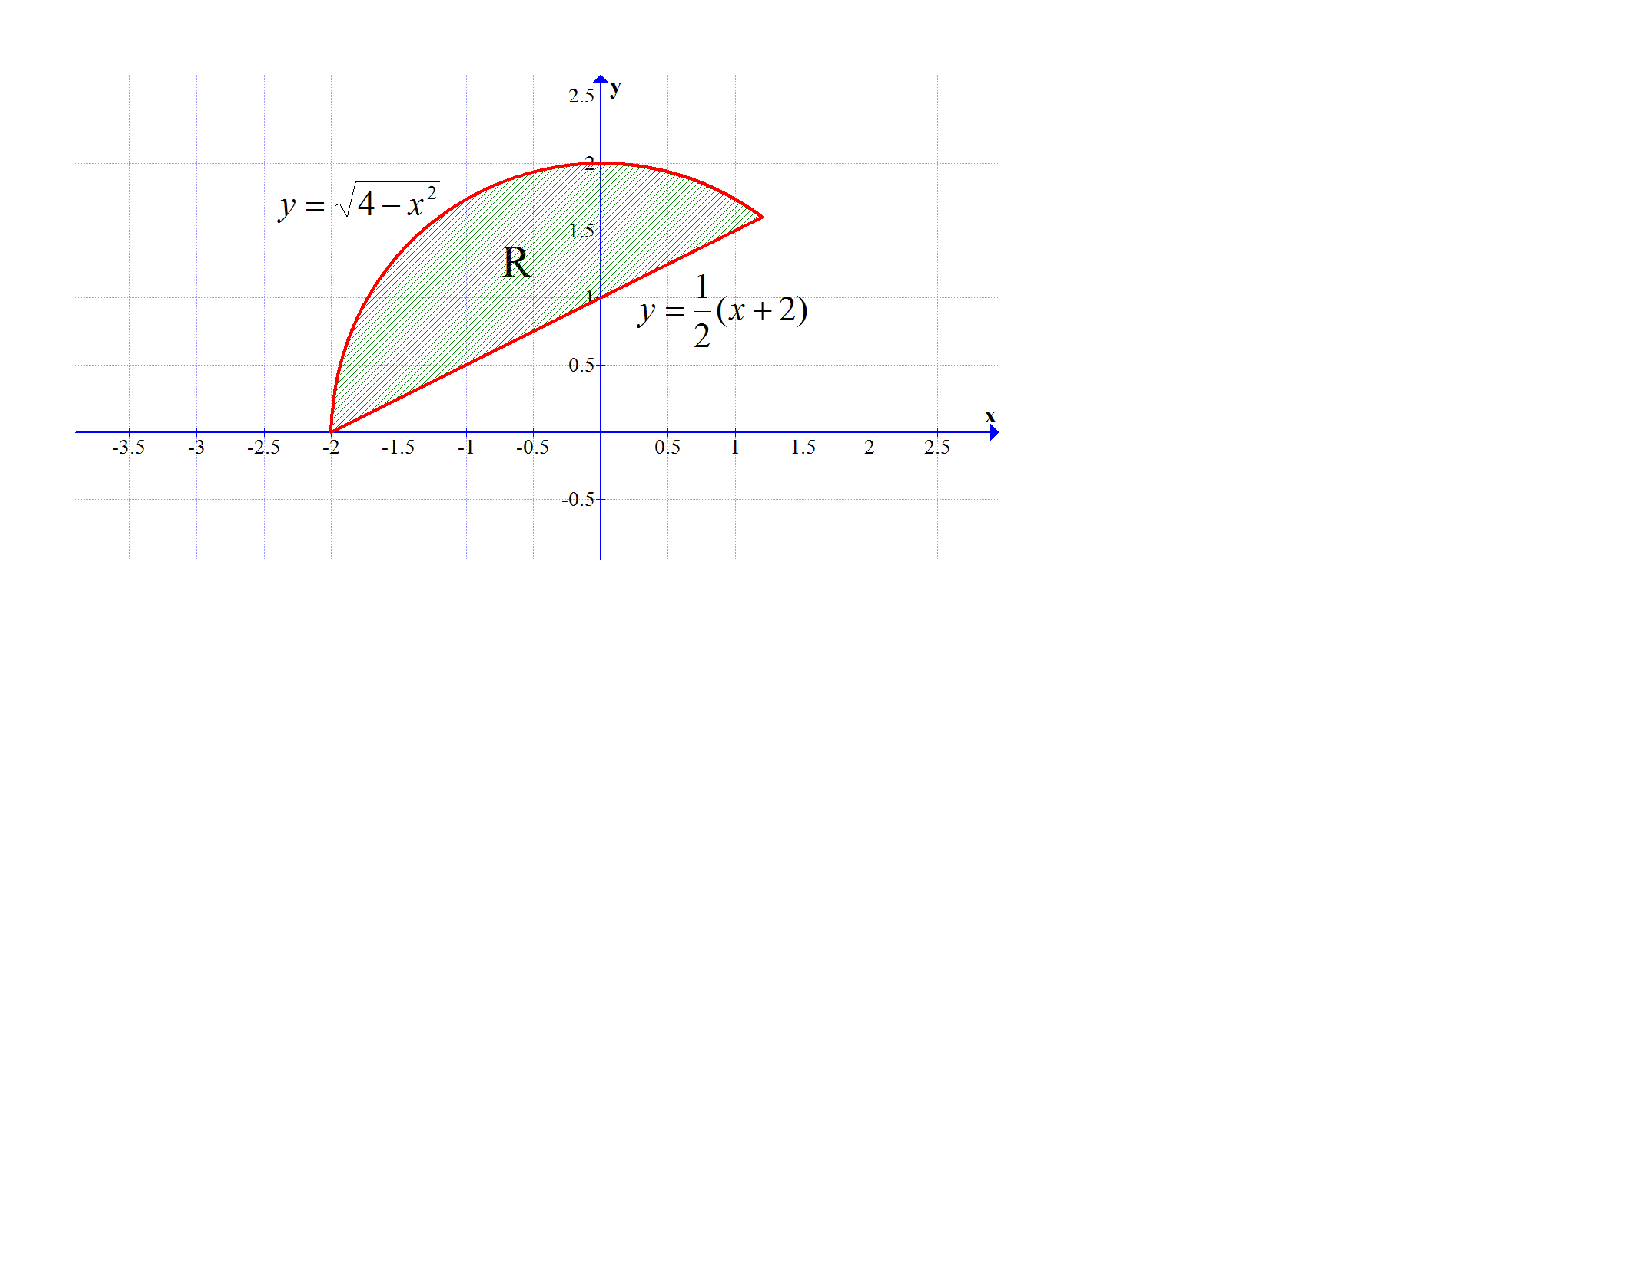
\includegraphics[scale=0.5]{int2.pdf}
\end{center}

\begin{enumerate}

\item Set up $\iint \limits_{R} f(x,y) \,dA$ with the order of integration as $\,dy\,dx$

\ifans{\fbox{$\int_{-2}^{6/5} \int_{\frac{1}{2}(x+2)}^{\sqrt{4-x^2}} f(x,y) \,dy \,dx$}} \fi

\item Set up $\iint \limits_{R} f(x,y) \,dA$ with the order of integration as $\,dx\,dy$

\ifans{\fbox{$\int_{0}^{8/5} \int_{-\sqrt{4-y^2}}^{2y-2} f(x,y) \,dx \,dy + \int_{8/5}^{2} \int_{-\sqrt{4-y^2}}^{\sqrt{4-y^2}} f(x,y) \,dx \,dy$}} \fi

\end{enumerate}

\end{enumerate}

\noindent {\bf For problems 3-7, evaluate the iterated integral.  For some problems, it may be helpful to switch the order of integration.}

\begin{enumerate}
\setcounter{enumi}{2}
\item $\int_1^2 \int_{-x}^x \left(y^2+3xy+x^2\right) \,dy \,dx$

\ifans{\fbox{10}} \fi

\item $\int_0^{\pi/3} \int_0^{\sin{x}} y\cos{x}\,dy\,dx$

\ifans{\fbox{$\frac{\sqrt{3}}{16}$}} \fi

\item $\int_0^1 \int_0^{x^3} \sqrt{1-x^4} \,dy \,dx$

\ifans{\fbox{$\frac{1}{6}$}} \fi

\item $\int_0^1 \int_y^1 \sqrt{1-x^2} \,dx \,dy$

\ifans{\fbox{$\frac{1}{3}$}} \fi

\item $\int_0^{\sqrt{\pi}/2} \int_{2y}^{\sqrt{\pi}} \sin{\left(x^2\right)}\,dx \,dy$

\ifans{\fbox{$\frac{1}{2}$}} \fi

\item Evaluate $\iint \limits_{R} \left(4x-3y\right) \,dA$ where $R$ is the region enclosed by the circle $x^2+y^2=1$.

\ifans{\fbox{0}} \fi

\item Evaluate $\iint \limits_{R} xy^2 \,dA$ where $R$ is the trianglar region enclosed by $y=3x$, $y=\frac{x}{2}$, and $y=1$.

\ifans{\fbox{$\frac{7}{18}$}} \fi

\item Let $R$ be the region enclosed by $y=x^2$ and $y=2x+3$.

\begin{enumerate}

\item Set up a double integral (or double integrals) with the order of integration as $\,dy\,dx$ which represents the area of $R$.

\ifans{\fbox{$\int_{-1}^3 \int_{x^2}^{2x+3} 1 \,dy\,dx$}} \fi

\item Set up a double integral (or double integrals) with the order of integration as $\,dx\,dy$ which represents the area of $R$.

\ifans{\fbox{$\int_{0}^1 \int_{-\sqrt{y}}^{\sqrt{y}} 1 \,dx\,dy+\int_1^9 \int_{\frac{1}{2}y-\frac{3}{2}}^{\sqrt{y}} 1 \,dx\,dy$}} \fi

\item Compute the area of $R$.

\ifans{\fbox{$\frac{32}{3}$}} \fi

\end{enumerate}

\item Use a double integral to find the volume of the solid in the first octant which is enclosed by the surface $3x+6y+2z=12$ and the coordinate planes.

\ifans{\fbox{8}} \fi

\item Consider the solid that enclosed by the cylinder $\frac{x^2}{9}+y^2=1$ and the planes $z=0$ and $x+2y+z=4$.  Use a double integral to compute the volume of this wedge.

\ifans{\fbox{$12\pi$; Detailed Solution: \textcolor{blue}{\href{http://www.math.drexel.edu/classes/Calculus/resources/Math200HW/Solutions/17_200_Double_Int_II_12.pdf}{Here}}}} \fi

\item Let $R$ be the region in the first quadrant of the $xy$ plane which is enclosed by $y=\sqrt{x}$, $x=0$ and $y=1$.  Compute the volume of the solid which is bounded above by $z=xe^{x/y^2}$ and has $R$ as its base.

\ifans{\fbox{$\frac{1}{5}$; Detailed Solution: \textcolor{blue}{\href{http://www.math.drexel.edu/classes/Calculus/resources/Math200HW/Solutions/17_200_Double_Int_II_13.pdf}{Here}}}} \fi

\end{enumerate}

\end{document}